\documentclass[varwidth=true, border=2pt]{standalone}
\usepackage{tkz-euclide}

\begin{document}
\usetkzobj{all}
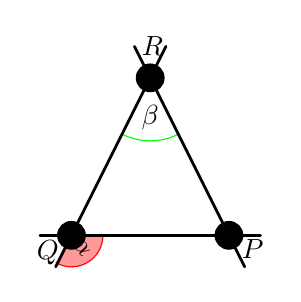
\begin{tikzpicture}
    \tkzSetUpPoint[shape=circle,size=10,color=black,fill=black]
    \tkzSetUpLine[line width=1]
    \tkzDefPoints{0/0/Q, 2/0/P, 1/2/R}


    \pgfmathsetmacro{\firstAngle}{0}
    \pgfmathsetmacro{\secondAngle}{-120}
    \path[draw,red, fill=red!40] (Q) -- ++(\firstAngle:.4) arc[start angle=\firstAngle, delta angle=\secondAngle,radius=.4];

    \tkzMarkAngle[arc=l,size=0.8cm,color=green,fill=green!20](Q,R,P)
    \path[draw] ++(-50:.2) node[rotate=-50] {$\alpha$};
    \node at (1,1.5) {$\beta$};
    \tkzDrawLine(Q,P)
    \tkzDrawLine(Q,R)
    \tkzDrawLine(P,R)
    \tkzDrawPoints(P,Q,R)
    \node at ($(R) + (0.03,0.4)$)    {$R$}; %top
    \node at ($(Q) + (-0.3,-0.22)$)  {$Q$}; %left
    \node at ($(P) + ( 0.3,-0.18)$)  {$P$}; %right
\end{tikzpicture}
\end{document}
